\documentclass[conference]{IEEEtran}
\usepackage[utf8]{inputenc}
\usepackage[T1]{fontenc}
\usepackage{cite,amsmath,amssymb,booktabs,graphicx,array,url}
\usepackage[hidelinks]{hyperref}
\graphicspath{{figures/}}
\title{Open-Weight Patient-to-Criterion Screening:\\Supervised Adaptation and Verified Transformer Inference}
\author{\IEEEauthorblockN{Muhammad Abdullah}
\IEEEauthorblockA{Student ID: 23i-0509\\FAST National University of Computer and Emerging Sciences\\Islamabad, Pakistan\\\texttt{i230509@isb.nu.edu.pk}}}
\begin{document}\maketitle
\begin{abstract}
Clinical-trial screening requires distinguishing explicit patient facts from missing information and checking inclusion and exclusion criteria separately. This work presents TrialLens, a local prototype using Qwen2.5-0.5B-Instruct adapted with LoRA on the mandatory TrialGPT Criterion Annotations dataset. A deterministic split assigns 37 patients to training, eight to validation, and eight to test. On 206 held-out criteria, the adapted model achieves 0.670 accuracy, 0.398 macro-F1, and 0.483 evidence sentence micro-F1; the unchanged base checkpoint achieves zero category accuracy under the structured-output parser. Explicit cached greedy decoding matches an uncached reference in six final Tesla T4 cases. Tiled online-softmax attention agrees numerically with a materialized reference while reducing longer-sequence allocation at substantial runtime cost. A custom greedy speculative decoder matches ordinary outputs in two cases but accepts no draft proposals and is slower. A browser interface displays criterion predictions, exact cited text, measured comparisons, and downloadable reports. Weak rare-category performance, exclusion evidence recall of 0.125, and an irrelevant citation in a synthetic demonstration limit reliability. This system is an educational screening prototype, not a clinical enrollment decision tool.
\end{abstract}
\begin{IEEEkeywords}clinical trial matching, Transformer, LoRA, evidence retrieval, KV cache, online softmax, speculative decoding\end{IEEEkeywords}
\section{Introduction and Problem Statement}

Trial eligibility matching requires reasoning over each individual inclusion or exclusion criterion and grounding a decision in specific patient-note sentences. Missing evidence must remain distinct from proof of failure. The criterion-level task is not a separately labeled patient--trial outcome. This work implements a small autoregressive model that generates both the expert category and evidence sentence IDs, using only the mandated annotations.
Given numbered note $p$, criterion type $t$, and text $c$, the objective is $(p,t,c)\mapsto(y,E)$, where $y$ is a preserved expert category and $E$ is a set of patient-sentence IDs. The contributions are a fixed-split supervised adaptation and audit pipeline, explicit cache/attention/speculative algorithms with measured correctness and efficiency, and a browser application for evidence inspection and export. The reported experiments distinguish predictive quality, text-origin verification, and inference performance because success in one does not establish success in the others.
\section{Related Work}

TrialGPT decomposes matching into trial retrieval, criterion-level reasoning, and patient-level ranking, and motivates preserving criterion granularity \cite{jin2024trialgpt}. The Transformer uses self-attention and autoregressive decoding \cite{vaswani2017attention}. LoRA freezes pretrained weights while training low-rank updates, reducing trainable parameter count \cite{hu2021lora}. FlashAttention demonstrates exact tiled attention with reduced memory traffic, while also showing why an IO-aware GPU implementation matters \cite{dao2022flashattention}. Long-context studies find that relevant facts can be missed depending on position, so a nominal context window alone does not guarantee robust evidence use \cite{liu2024lost}. Qwen2.5 and SmolLM2 supply two small open-weight decoder candidates \cite{qwenmodel,allal2025smollm}.

Speculative decoding uses a cheaper draft and target verification to reduce serial target calls when proposals are accepted~\cite{leviathan2023speculative,chen2023speculative}. We implement its deterministic greedy case, not probabilistic rejection sampling. The cited literature motivates mechanisms; no published TrialGPT accuracy or speedup is treated as a result of this implementation.
\section{Materials and Methods}

\subsection{Dataset and split}
The NCBI TrialGPT Criterion Annotations dataset has 1,015 criterion annotations from 53 patients in the executed dataset release \cite{trialgptdataset}. We sort the unique IDs and shuffle with NumPy \texttt{default\_rng(42)}, allocating 37, 8, and 8 patients to train, validation, and test. The script exports patient IDs, row counts, and leakage checks. Input fields are note, criterion type, and criterion text. Targets are expert eligibility and expert sentence IDs. All GPT-4-generated fields and correctness judgments are excluded.
\subsection{Architecture choice}
We selected Qwen2.5-0.5B-Instruct (approximately 0.49B parameters; Apache-2.0; decoder-only causal Transformer; native Qwen2 tokenizer; model card reports context up to 32,768 tokens). BF16 weights alone occupy about 0.98 GB decimal; actual training memory also includes activations, optimizer state for adapters, gradients, and cache. LoRA with short 2,048-token sequences and checkpointing is intended for a free 8--16 GB GPU. SmolLM2-360M-Instruct (0.36B, Apache-2.0, decoder-only, 8K context) is a smaller alternative, but Qwen provides more context headroom for longer notes. The downloaded base checkpoint was approximately 988 MB; training used a free Colab Tesla T4 with mixed precision and gradient checkpointing; later inference benchmarks used FP32. Peak GPU memory was not recorded, so no measured peak-memory claim is made.
\subsection{Preprocessing and output}
The note's numbered sentences are retained. The prompt includes exactly the three required inputs. The target is a JSON object with keys \texttt{eligibility} and \texttt{evidence\_sentence\_ids}; for example, category \texttt{included} with IDs \texttt{[2]}. The six supported categories are included, not included, excluded, not excluded, not enough information, and not applicable. Evidence uses original sentence IDs, including zero-based IDs when present. The tokenizer is native to Qwen2.5. Training is limited to 2,048 total tokens, preserving the beginning of the prompt and potentially dropping later evidence. Each record logs original token count, used count, and truncation flag. Evaluation reserves up to 128 generation tokens from that budget. The held-out test truncation fraction is 0.000 for both base and adapted models; longer future notes may still lose relevant evidence.
\subsection{Fine-tuning objective and configuration}
We use causal next-token cross-entropy over target JSON tokens; prompt token labels are masked with -100. LoRA uses rank 8, alpha 16, dropout 0.05, and attention projection modules. Executed settings were AdamW, learning rate $2\times10^{-4}$, 3 epochs, microbatch 1, accumulation 8, warmup 5\%, weight decay 0.01, seed 42, and best validation-loss checkpoint. Training took 622.75 s; full-run mean training loss was 0.1860 and validation loss was 0.1209. The full training history is in the submission artifact archive. Greedy generation uses no sampling and a 128-token output cap for both base and adapted model.

The prompt uses plain concatenated instructions rather than a chat template. An audit of adapter tensor shapes gives 1,081,344 trainable parameters. For projection $W$, LoRA computes $Wx+(\alpha/r)BAx$ with frozen $W$~\cite{hu2021lora}. For target tokens $z_{1:m}$, the objective is
\begin{equation}
\mathcal{L}=-\frac{1}{m}\sum_{j=1}^{m}\log P_{\theta,\phi}(z_j\mid p,t,c,z_{<j}),
\end{equation}
where pretrained weights $\theta$ are frozen and adapter weights $\phi$ are optimized. The best validation-loss checkpoint is update 228 of 228 total optimizer updates. Training and validation preprocessing logs report zero truncation. Exact original library versions and every Colab runtime patch were not archived; version ranges in the environment specification do not constitute a complete lockfile.

\begin{table}[t]\centering
\caption{Prescribed patient split reproduced by the saved manifest.}
\label{tab:split}
\begin{tabular}{lrr}\toprule Partition & Patients & Criteria\\\midrule
Train & 37 & 603\\Validation & 8 & 206\\Test & 8 & 206\\\midrule Total & 53 & 1,015\\\bottomrule
\end{tabular}\end{table}
Table~\ref{tab:split} shows that equal patient counts need not imply equal annotation counts. Every annotation for a patient stays in one partition. Input fields are whitelisted in the preparation script, rather than only dropping a few known model-generated columns.

\begin{table*}[t]\centering
\caption{Model candidates. Weight memory is an estimate ($2P$ or $4P$ bytes), not a measured process peak. Decimal GB are used.}
\label{tab:models}
\begin{tabular}{lrrrrrl}\toprule Candidate & Parameters & Layers & Q/KV heads & Context & FP16 / FP32 GB & License\\\midrule
Qwen2.5-0.5B-Instruct~\cite{qwenmodel,qwenconfig} & $\approx$0.49B & 24 & 14/2 & 32,768 & 0.98 / 1.96 & Apache-2.0\\
SmolLM2-360M-Instruct~\cite{smolmodel,smolconfig} & $\approx$0.36B & 32 & 15/5 & 8,192 & 0.72 / 1.44 & Apache-2.0\\\bottomrule
\end{tabular}\end{table*}
Table~\ref{tab:models} supports a practical resource comparison, not a clinical-quality comparison; SmolLM2 was not trained or scored here. Qwen's native window is larger than the configured experiment budget. The selected model has hidden size 896, feed-forward size 4,864, 24 layers, and vocabulary size 151,936~\cite{qwenconfig}. It uses GQA, RoPE, RMSNorm, SwiGLU, residual connections, and tied embeddings~\cite{qwenmodel}. Figure~\ref{fig:architecture} links this architecture to the supervised and browser pipelines.

\begin{figure*}[t]\centering
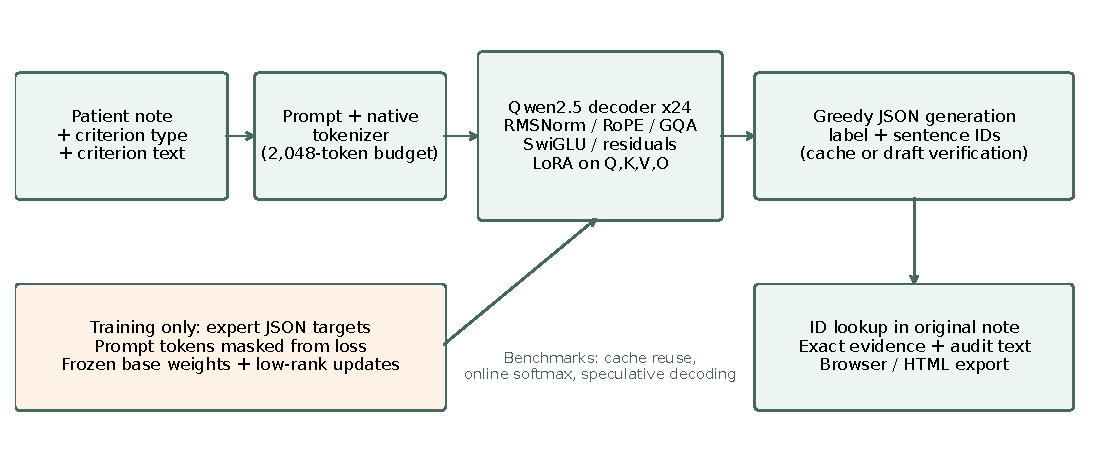
\includegraphics[width=\textwidth]{system_architecture.pdf}
\caption{Implemented system and training flow. Only expert JSON targets supervise LoRA. Evidence text is retrieved from the original note after generation. The attention microbenchmark is an independent experiment rather than a replacement kernel inside the target model.}
\label{fig:architecture}\end{figure*}
\subsection{Prediction and Evidence Pipeline}

The evaluator preserves the expert label strings rather than mapping them into binary decisions. It returns criterion text and type, predicted category, cited sentence IDs, verbatim sentence text for IDs found in the numbered patient note, unmatched IDs, and a deterministic audit explanation. The explanation quotes only the cited text; when no sentence is cited, it explicitly states that missing evidence is not proof of either outcome. The machine-readable per-record schema is saved with the evaluation JSON. Historical Task 1 logs lacked criterion text and evidence text, so Task 2 analysis below re-aggregates their existing predictions without rerunning test inference.

\subsection{Explicit KV-Cached Generation}


We implemented the greedy decoding loop in \texttt{src/cache\_decode.py} rather than relying only on a high-level generation switch. The cached implementation performs one prompt prefill with \texttt{use\_cache=True}, selects the next token by argmax, and then feeds one token per forward pass while carrying the returned \texttt{past\_key\_values}. The reference implementation uses \texttt{use\_cache=False} and recomputes the entire prompt-plus-generated prefix at each step. Both implementations apply identical greedy argmax selection, EOS handling, and input IDs.

Qwen2.5 uses rotary positional embeddings. Prompt positions follow the model's zero-based positions; cached decoding explicitly assigns each new token position $L+j$, where $L$ is prompt length and $j$ is its zero-based generated-token index. The attention mask grows by one visible position per step, while the model's causal mask disallows attending to future positions. Benchmark prompts are unpadded, so no padding offset is needed. The key/value cache grows linearly with generated sequence length. Differences in floating-point kernel order can alter an argmax when top logits are nearly tied, so the benchmark records per-token agreement and exact-sequence agreement.


For batch $B$, layers $N$, KV heads $H_{kv}$, head dimension $d$, sequence length $S$, and $b$ bytes per element, the basic cache storage estimate is $M_{KV}=2BNH_{kv}dSb$. For Qwen at batch one and FP32, this is approximately 24 KiB per cached token before other tensors. LoRA reduces trainable optimizer state but does not remove activations, base weights, or cache storage.
\subsection{Tiled Attention and Online Softmax}


We implemented a materialized scaled dot-product attention reference and a tiled online-softmax variant in \texttt{src/online\_attention.py}. For each query tile, the tiled method visits key/value tiles and maintains a running maximum $m$, normalization sum $l$, and weighted-value accumulator $a$. For score tile $S$, it updates $m'=\max(m,\max(S))$, rescales the previous state by $\alpha=\exp(m-m')$, then adds the shifted tile exponentials to $l$ and their product with values to $a$. The output is $a/l$. This is numerically stable because exponentials are evaluated after subtracting the current maximum. Half and bfloat16 inputs are accumulated in float32. Fully masked rows return zero.

The reference and tiled paths accept boolean visibility masks and additive score masks, including negative infinity for blocked positions. Causal masking allows each query to attend only to its current and preceding keys. For a shorter query suffix over a longer KV sequence, positions are bottom-right aligned. Tests exercise causal attention, additive and boolean masks, fully masked rows, uneven tile boundaries, and suffix queries; outputs agree with the reference and PyTorch SDPA within tight float64 tolerances. The test command and general benchmark command are documented in the README.


The reference computes $O=\operatorname{softmax}(QK^\top/\sqrt{d}+M)V$. For each new tile $S$, the online recurrence is
\begin{align}
m'&=\max(m,\operatorname{rowmax}(S)),\\
P&=\exp(S-m'),\quad \beta=\exp(m-m'),\\
\ell'&=\beta\ell+\operatorname{rowsum}(P),\\
a'&=\beta a+PV,\quad O=a'/\ell'.
\end{align}
Fully masked rows are explicitly returned as zero to avoid undefined infinity subtraction. This attention implementation is a separate controlled experiment; it is not injected into the fine-tuned target's forward pass.
\subsection{Greedy Speculative Decoding}


We implement greedy speculative decoding in \texttt{src/speculative\_decode.py}. The draft proposes up to $k$ tokens autoregressively. The target evaluates the complete candidate block in one forward pass. Candidate $i$ is accepted only when it equals the target's greedy argmax at that position. At the first mismatch, the target's argmax replaces the rejected token; the draft and target caches are cropped to the accepted prefix and both are advanced with the replacement token. If all candidates match, the target's final verification logits produce an extra greedy bonus token. EOS and output-length limits terminate the process without adding unrequested tokens.

The target is Qwen2.5-0.5B-Instruct with the trained LoRA adapter merged into its base weights. We form a smaller draft by copying this merged model and retaining only its first two of 24 decoder layers. The draft shares the target's embeddings, final normalization, output head, vocabulary, and tokenizer, while its retained layers inherit the target's adapted weights. This avoids token-ID remapping and duplicate vocabulary-scale weights. It may still predict poorly because most decoder layers are omitted, and a higher rejection rate can erase the savings from fewer target calls.


The explicit decoding loop is:
\begin{enumerate}
\item Prefill target and draft with the same accepted history.
\item Draft up to four tokens autoregressively and update the draft cache.
\item Verify the candidate block in one target call. Previous target logits score the first candidate; shifted block logits score later candidates.
\item Accept the matching greedy prefix. On rejection, crop both caches to that prefix, emit the target correction, and advance both caches with it.
\item If the full block matches, emit the target bonus token when allowed and synchronize both caches. Stop at EOS or the output cap.
\end{enumerate}
The smaller draft is a feasible compatibility baseline, not a separately optimized model. Its retained layers are not trained to compensate for the removed layers.
\subsection{Browser Application Workflow}

The local browser application is implemented with a Python HTTP server and a standalone responsive HTML/CSS/JavaScript interface. The user enters a patient record, adds inclusion or exclusion criteria, and selects cached greedy or the custom two-layer speculative decoder. The model uses the trained Qwen2.5-0.5B-Instruct LoRA adapter and runs locally on CUDA when available or on CPU otherwise. Each criterion output retains its predicted category, exact source sentence IDs and text, a note-grounded explanation, generation latency, and truncation status. Sentence IDs are resolved against numbered sentences in the supplied record; unmatched citations are not displayed as verified evidence. The interface preserves ``not enough information'' and ``not applicable,'' warns when the prompt exceeds the configured window, and never treats absent evidence as proof of either eligibility outcome. A downloadable and printable HTML screening report carries the educational-prototype notice. The separate inference laboratory presents the measured Task 3 and Task 5 comparisons; the speculative results explicitly show that token correctness did not produce a speedup for the low-acceptance draft. The app is started on Windows by double-clicking \texttt{setup\_and\_run.bat}; the script prepares the environment and opens the locally hosted browser page. Patient text is not persisted or written to server access logs. The system remains a research screening prototype and is not a clinical enrollment decision tool.

The app preserves the criterion and later text by left-truncating overly long prompts, whereas training and benchmark evaluation preserve the beginning. The UI reports that difference through truncation warnings and token counts. Neither direction guarantees preservation of relevant evidence. Results remain in the browser until the user exports them. The interface displays no separately ground-truth-labeled patient--trial enrollment verdict.
\section{Experimental Setup and Metrics}

The scripts evaluate base and adapted checkpoints on identical validation examples and the same held-out test examples. Classification results include accuracy, macro-F1, class precision/recall/F1, and confusion matrix. Evidence is exact sentence-ID set matching with micro precision, recall, and F1. Empty-set treatment follows corpus-level sentence-ID counts, detailed below. Invalid JSON is mapped to the “invalid” label and is visible in the per-example prediction log. The Colab run used a Tesla T4; training took 622.75 s (3 epochs). Test generation averaged 3.594 s/criterion for the base model and 0.984 s/criterion for LoRA. The test split contains 206 criteria from 8 patients, with no reported truncation.

Macro-F1 is computed over the union of gold and predicted labels in each group, with zero for undefined precision or recall; overall and criterion-type macro scores may therefore average different observed class sets. No test examples support the excluded class, so its held-out performance is not estimable. Inference benchmarks use validation-derived prompt IDs, not held-out test cases. The fixed-length prompt construction is a controlled workload, not a random sample of clinical inputs.

For sentence sets $E_i$ and predictions $\hat E_i$, $TP=\sum_i|E_i\cap\hat E_i|$, $P=TP/\sum_i|\hat E_i|$, $R=TP/\sum_i|E_i|$, and $F1=2PR/(P+R)$. Empty-evidence policy is corpus-level: a both-empty record contributes no sentence IDs; it does not add a separate true positive. If both totals are empty for the entire group, all three scores are one. A one-sided empty total receives zero for the affected metric; F1 is zero if $P+R=0$.

Cache and speculative benchmarks use eager attention and FP32 on both compared paths, synchronize CUDA for timing, and warm up before recording results. Prefill and decode are timed separately. Decode throughput divides actual output tokens by decode time; overall throughput additionally includes prefill. Output lengths are caps, with EOS permitted. The 256-token cache cases emit seven tokens, explaining similar results for caps 16 and 32. Peak CUDA allocation includes weights and live tensors; incremental peak relative to pre-run allocation is retained in JSON. Model loading is excluded. Decoding is measured once per configuration, whereas attention reports medians over ten timed iterations. SDPA's dispatched kernel was not pinned or recorded, so no specific fused-backend claim is made.
\section{Results and Discussion}
\subsection{Training Dynamics and Predictive Performance}
Figure~\ref{fig:training} plots the actual archived training history. Validation losses at updates 76, 152, and 228 are 0.1531, 0.1232, and 0.1209. The last epoch gives a smaller gain than the first two; the selected checkpoint is update 228. The trainer's 0.1860 training loss is a full-run mean, not the final batch loss. Low JSON-token loss must not be equated with clinical reliability.
\begin{figure}[t]\centering
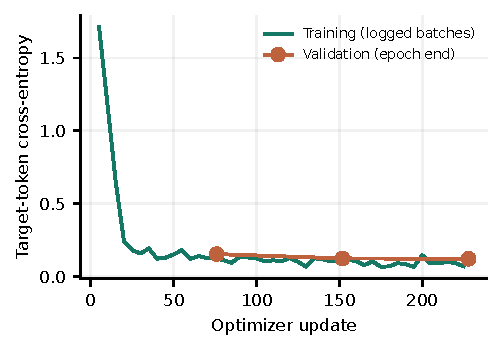
\includegraphics[width=\columnwidth]{training_curve.pdf}
\caption{Logged training batch losses and epoch-end validation losses. Validation was measured at three checkpoints only; connecting lines do not imply intermediate observations.}
\label{fig:training}\end{figure}

\begin{table}[t]\centering\caption{Validation and held-out test results. Evidence scores are micro-averaged over exact sentence-ID sets.}\label{tab:prediction}\begin{tabular}{llcc}\toprule Split & Metric & Base & LoRA\\\midrule Validation & Accuracy & 0.000 & 0.718\\Validation & Macro-F1 & 0.000 & 0.354\\Validation & Evidence micro-F1 & 0.021 & 0.441\\Test & Accuracy & 0.000 & 0.670\\Test & Macro-F1 & 0.000 & 0.398\\Test & Evidence micro-F1 & 0.043 & 0.483\\Test & Truncation fraction & 0.000 & 0.000\\Test & Mean generation (s/criterion) & 3.594 & 0.984\\\bottomrule\end{tabular}\end{table}
Table~\ref{tab:prediction} shows that fine-tuning improved label and evidence matching on validation and held-out test data. The base model generated many free-form or dictionary-like outputs instead of the required JSON label, producing zero accuracy and macro-F1; this is an output-format failure as well as a model-quality issue. Fine-tuning improved held-out accuracy to 0.670 and evidence micro-F1 to 0.483, while the test macro-F1 of 0.398 indicates uneven performance across classes. Validation and test results differ, which is expected for a small split of only eight patients in each. No inputs were truncated in either evaluation. Fine-tuned per-example predictions, aggregate base metrics, training history, split manifest, and adapter are packaged in results/task1_submission_artifacts.zip; unstructured base generations are redacted from the public bundle because they may quote patient-note text. The base and adapted generation latency figures are measured means; multiplying by 206 implies approximately 740 s and 203 s for each test pass, respectively.
\subsection{Criterion-Type and Evidence Error Analysis}
\begin{table*}[t]\centering\caption{Held-out fine-tuned results by criterion type. Evidence metrics use exact sentence-ID sets.}\label{tab:bytype}\begin{tabular}{lrrrrrr}\toprule Group & $n$ & Accuracy & Macro-F1 & Evidence P & Evidence R & Evidence F1 \\\midrule Overall & 206 & 0.670 & 0.398 & 0.525 & 0.447 & 0.483 \\
Inclusion & 75 & 0.640 & 0.339 & 0.543 & 0.613 & 0.576 \\
Exclusion & 131 & 0.687 & 0.271 & 0.400 & 0.125 & 0.190 \\\bottomrule\end{tabular}\end{table*}
Table~\ref{tab:bytype} shows more even inclusion than exclusion evidence retrieval: exclusion evidence recall was only 0.125. Per-class scores and confusion matrices for both the base and adapted models are included in \texttt{results/task2\_error\_analysis.json}. For the adapted model, the overall per-class (precision, recall, F1, support) values were included (0.654, 0.630, 0.642, 27), not applicable (0, 0, 0, 15), not enough information (0.620, 0.470, 0.534, 66), not excluded (0.692, 0.989, 0.814, 91), and not included (0, 0, 0, 7). Zero F1 on not applicable and not included shows that retaining those categories in the schema did not ensure that the model learned to predict them.


Table~\ref{tab:classes} supplies per-class metrics for the same groups. All gold baseline classes have zero precision, recall, and F1 under the structured parser. Figure~\ref{fig:confusion} visualizes fine-tuned confusion counts overall and separately by inclusion/exclusion. Empty NA and NINC prediction columns expose category collapse even though those strings remain in the output schema.
\begin{table}[t]\centering
\caption{Fine-tuned per-class test scores. INC=included; NINC=not included; NEX=not excluded; NA=not applicable; NEI=not enough information.}
\label{tab:classes}\small\begin{tabular}{llrrrr}
\toprule
Group & Class & P & R & F1 & $n$\\
\midrule
Overall & INC & 0.654 & 0.630 & 0.642 & 27\\
Overall & NA & 0.000 & 0.000 & 0.000 & 15\\
Overall & NEI & 0.620 & 0.470 & 0.534 & 66\\
Overall & NEX & 0.692 & 0.989 & 0.814 & 91\\
Overall & NINC & 0.000 & 0.000 & 0.000 & 7\\
\midrule
Inclusion & INC & 0.654 & 0.630 & 0.642 & 27\\
Inclusion & NA & 0.000 & 0.000 & 0.000 & 3\\
Inclusion & NEI & 0.633 & 0.816 & 0.713 & 38\\
Inclusion & NINC & 0.000 & 0.000 & 0.000 & 7\\
\midrule
Exclusion & NA & 0.000 & 0.000 & 0.000 & 12\\
Exclusion & NEI & 0.000 & 0.000 & 0.000 & 28\\
Exclusion & NEX & 0.692 & 0.989 & 0.814 & 91\\
\bottomrule
\end{tabular}

\end{table}
\begin{figure*}[t]\centering
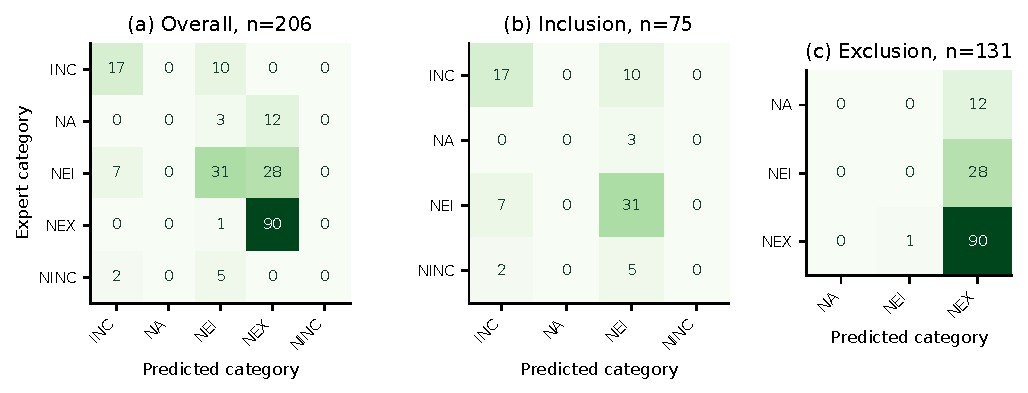
\includegraphics[width=\textwidth]{confusion_matrices.pdf}
\caption{Test confusion matrices, raw counts. Rows are expert categories; columns are predictions. Class abbreviations follow Table~\ref{tab:classes}. All 28 exclusion NEI cases and all 12 exclusion NA cases become NEX.}
\label{fig:confusion}\end{figure*}
The evidence evaluator computes corpus-level micro precision, recall, and F1 over sentence-ID sets. If both gold and predicted evidence are empty for the whole group, all three metrics are 1; if only one side is empty, the affected metric is 0. Of 66 gold not-enough-information records, the model preserved that category in 31 and made a definitive prediction in 35. All 28 exclusion records with insufficient information were predicted as not excluded; 26 had no cited evidence and two did. Two opposing inclusion errors predicted included where the gold category was not included; one example (patient sigir-201410) had no gold evidence but the model cited IDs 0 and 1. These are prediction-vs-annotation conflicts, not verified contradictions in the underlying patient record. The full representative errors and counts are in the analysis JSON. The current evaluator attaches evidence text for future runs, but no new held-out inference was performed after this pipeline change.

Of 206 test records, 145 have no gold evidence and 145 have no predicted evidence, but only 128 are empty on both sides. Seventeen gold-empty records receive citations and 17 gold-nonempty records receive none. Matching empty-set totals therefore does not imply correct retrieval. Historical representative-error logs omit criterion and evidence text; these are prediction-versus-annotation conflicts rather than independently verified clinical contradictions. The zero baseline scores are partly a schema failure; they do not show that the pretrained model has no task knowledge. Shorter, better-formed adapted outputs may also explain its lower generation latency rather than an inherent LoRA acceleration.
\subsection{KV Cache Agreement and Performance}
The reproducible comparison is implemented in \texttt{src/benchmark\_cache.py}. It verifies actual cache sequence length after prefill and every incremental update, and measures prefill latency, decode latency, tokens per second, and peak CUDA allocation for 64/256/512-token prompts and 16/32-token output caps. We measured the fine-tuned Qwen2.5-0.5B model on a Tesla T4 with float32 computation, eager attention on both paths, and four warmup tokens per path. The complete measurements are archived in \texttt{results/cache\_benchmark\_final.json}; Table~\ref{tab:cache-final} summarizes them. All six tested cached and uncached greedy sequences matched token for token. The earlier exploratory bfloat16 run with unspecified attention backend diverged on the 64- and 256-token prompts. The successful rerun changed backend and dtype together, so it establishes exact agreement under the final settings but cannot attribute the earlier mismatch to only one cause.

\begin{table*}[t]
\centering
\caption{Tesla T4 KV-cache benchmark. Prefill/decode are seconds, throughput is generated tokens/s, and peak allocation includes the model/runtime (GiB). Paired values are cached/reference.}
\label{tab:cache-final}
\small
\begin{tabular}{rrccccc}
\hline
Prompt & Cap & Exact match & Prefill & Decode & Throughput & Peak memory \\
\hline
64 & 16 & Yes & 0.055 / 0.046 & 0.662 / 0.746 & 24.18 / 21.46 & 1.89 / 1.94 \\
64 & 32 & Yes & 0.050 / 0.066 & 1.385 / 1.523 & 23.10 / 21.01 & 1.89 / 1.96 \\
256 & 16 & Yes & 0.071 / 0.066 & 0.258 / 0.581 & 27.14 / 12.05 & 2.01 / 2.15 \\
256 & 32 & Yes & 0.074 / 0.067 & 0.260 / 0.585 & 26.93 / 11.96 & 2.01 / 2.15 \\
512 & 16 & Yes & 0.154 / 0.147 & 0.880 / 2.637 & 18.19 / 6.07 & 2.16 / 2.45 \\
512 & 32 & Yes & 0.151 / 0.149 & 1.372 / 5.495 & 23.33 / 5.82 & 2.16 / 2.47 \\
\hline
\end{tabular}
\end{table*}

Table~\ref{tab:cache-final} shows lower decode latency and peak allocation for cached decoding in every measured case. The throughput advantage is clearest for longer prompts: cached throughput is approximately 3.0--4.0 times the reference at 512 tokens. Short prompts show a smaller gain. These results cover one validation prompt per requested length on one T4, and therefore characterize this run rather than all inputs or GPU types. Peak allocation includes the resident model and runtime; incremental peak allocation is also retained in the JSON log.


Figure~\ref{fig:decoding}(a) plots the cap-32 throughput comparison. Prompt-dependent outputs and early EOS prevent interpreting the curve as a controlled repeated-trial scaling law. Figure~\ref{fig:decoding}(b) uses overall throughput including prefill for the speculative comparison; the timing definitions are deliberately distinguished.
\begin{figure*}[t]\centering
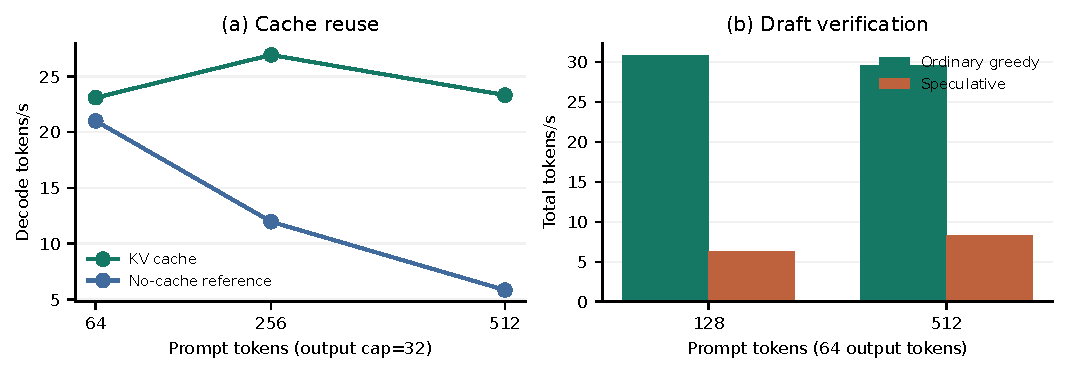
\includegraphics[width=\textwidth]{decoding_comparison.pdf}
\caption{T4 generation throughput. (a) Decode-only throughput for output cap 32, with EOS permitted. (b) Throughput including prefill for 64 generated tokens. Measurements cover one workload per requested length.}
\label{fig:decoding}\end{figure*}
\subsection{Tiled Attention Correctness and Efficiency}
Table~\ref{tab:attention-cpu} reports the small CPU comparison (batch 1, two heads, head dimension 16, float32; two timed iterations after one warmup); the complete measurements are in \texttt{results/attention\_benchmark\_cpu.json}. We also benchmarked on a Tesla T4 with batch 1, four heads, head dimension 32, float32, causal masking, 32-by-64 tiles, three warmups, and ten timed iterations. Table~\ref{tab:attention-t4} and \texttt{results/attention\_benchmark\_t4.json} report medians, maximum absolute error, and peak CUDA allocation. Every method passed the configured tolerance; tiled attention's maximum absolute errors were below $4.2\times10^{-7}$. At length 512, measured peak allocation was 30.83 MB for the reference and 10.38 MB for tiled attention. The tiled Python implementation was substantially slower, taking 89.22 ms versus 0.90 ms for the materialized reference at this length. This demonstrates the memory/runtime tradeoff for this implementation and run; allocation includes runtime and other live tensors, not just the score matrix.

\begin{table}[t]
\centering
\caption{CPU attention timing in milliseconds (float32).}
\label{tab:attention-cpu}
\begin{tabular}{rccc}
\hline
Length & Reference & Tiled online & PyTorch SDPA \\
\hline
32 & 2.16 & 3.68 & 0.15 \\
64 & 0.76 & 7.69 & 0.15 \\
\hline
\end{tabular}
\end{table}

\begin{table}[t]
\centering
\caption{Tesla T4 causal attention benchmark. Time is median milliseconds; memory is peak CUDA allocation in decimal MB.}
\label{tab:attention-t4}
\begin{tabular}{r l r r r}
\hline
Length & Method & Time (ms) & Peak (MB) & Max error \\
\hline
64 & Reference & 0.744 & 8.98 & 0 \\
64 & Tiled online & 1.773 & 8.88 & $3.58\times10^{-7}$ \\
64 & PyTorch SDPA & 0.070 & 8.75 & $5.96\times10^{-7}$ \\
256 & Reference & 0.727 & 14.37 & 0 \\
256 & Tiled online & 22.877 & 9.50 & $4.17\times10^{-7}$ \\
256 & PyTorch SDPA & 0.140 & 9.47 & $6.26\times10^{-7}$ \\
512 & Reference & 0.900 & 30.83 & 0 \\
512 & Tiled online & 89.215 & 10.38 & $3.87\times10^{-7}$ \\
512 & PyTorch SDPA & 0.250 & 10.49 & $7.15\times10^{-7}$ \\
\hline
\end{tabular}
\end{table}

The reference and tiled implementations are educational PyTorch code, not fused CUDA kernels. The tiled version dispatches several tensor operators and Python loop iterations per block; optimized attention kernels fuse score calculation, online normalization, and value accumulation while reducing memory traffic. This explains why our tiled method can use less peak allocation at longer lengths yet run much slower than both the materialized baseline and PyTorch SDPA. The T4 benchmark uses a single fixed shape and a short microbenchmark, so its timing should not be generalized to other workloads or GPUs.


Figure~\ref{fig:attention} compares attention time and allocation directly. At length 512, tiled allocation is about one third of the reference, but tiled latency is about 99 times greater. The Python loop and operator dispatch overhead demonstrate why the online-softmax algorithm alone does not guarantee fused-kernel performance.
\begin{figure*}[t]\centering
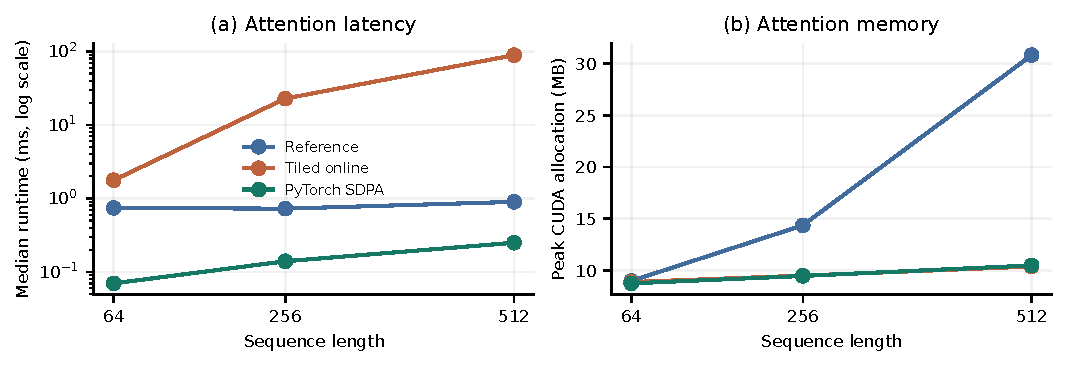
\includegraphics[width=\textwidth]{attention_comparison.pdf}
\caption{T4 median attention runtime (logarithmic axis) and peak CUDA allocation (decimal MB). The educational tiled implementation reduces longer-sequence allocation while adding substantial runtime.}
\label{fig:attention}\end{figure*}
\subsection{Speculative Decoding Correctness and Slowdown}
The unit tests verify all-accepted rounds, rejected-token correction, EOS handling, cache-length alignment, and exact equality with ordinary greedy on deterministic toy models. We additionally benchmarked the fine-tuned target on a Tesla T4 with eager attention and float32. Table~\ref{tab:specbench} reports cached ordinary greedy against the two-layer speculative draft for 64 output tokens. In both validation-prompt cases, generated token IDs matched exactly. The draft accepted 0 of 250 proposed tokens (0\%); each run had 64 rounds and 64 rejected rounds. Consequently, speculative decoding was slower: its total runtime was 10.170 s versus 2.076 s for a 128-token prompt, and 7.721 s versus 2.166 s for a 512-token prompt. The draft's additional serial forward passes explain the slowdown when proposals are consistently rejected. Peak CUDA allocation was also higher for speculative decoding, as it keeps draft and target caches: 2166.92 versus 2085.61 MiB at 128 input tokens, and 2624.08 versus 2320.78 MiB at 512. Decode throughput fell from 31.59 to 6.33 tokens/s and from 31.84 to 8.51 tokens/s, respectively. The full measured log is provided in \texttt{results/speculative\_benchmark\_t4.json}. These two validation cases establish correctness and document this draft's poor acceptance; they do not establish a speedup or generalize to other prompts or hardware.

\begin{table*}[t]
\centering
\caption{Tesla T4 greedy speculative decoding benchmark (64 generated tokens; validation prompts).}
\label{tab:specbench}
\begin{tabular}{r|rr|rr|rr|c}
\toprule
Input & \multicolumn{2}{c|}{Total time (s)} & \multicolumn{2}{c|}{Decode tok/s} & \multicolumn{2}{c|}{Peak MiB} & Exact\\
tokens & Greedy & Spec. & Greedy & Spec. & Greedy & Spec. & match\\
\midrule
128 & 2.076 & 10.170 & 31.59 & 6.33 & 2085.61 & 2166.92 & Yes\\
512 & 2.166 & 7.721 & 31.84 & 8.51 & 2320.78 & 2624.08 & Yes\\
\bottomrule
\end{tabular}
\end{table*}

Overall throughput including prefill is 30.82 versus 6.29 tokens/s at 128 input tokens and 29.54 versus 8.29 at 512. The speculative path is therefore about 4.90 and 3.56 times slower end to end. Zero acceptance forces one useful target correction per round while adding draft calls, verification, rollback, and resynchronization overhead. These real-model cases verify the exercised rejection path, while toy cases cover all-accepted rounds. A separately adapted draft and a wider prompt sample would be needed to investigate a useful speedup.
\subsection{Browser Demonstration and Report Export}
The browser workflow was exercised on 10 November 2026 with a synthetic patient and one inclusion and one exclusion criterion. Local CPU inference returned ``included'' for ECOG status in 10.70 s and ``not excluded'' for heart failure in 7.47 s. The report downloaded successfully and preserved the displayed citations and prototype notice. The ECOG prediction cited sentence 1 rather than the relevant sentence 2, demonstrating a model evidence-selection failure despite a functioning application pipeline. The exclusion citation correctly reproduced sentence 3. These examples verify application behavior and are not additional benchmark accuracy results. The demonstration report and verification notes are saved in the results directory.

\IfFileExists{figures/application_results.png}{
Figure~\ref{fig:app} shows an actual browser rerun of the same synthetic case. Its visible CPU times are 21.27 s and 9.47 s, rather than the earlier exported demonstration's 10.70 s and 7.47 s. Both runs return the same categories and citations. They are not pooled as a timing benchmark. Exact quotation preserves the erroneous ECOG citation rather than silently replacing it with sentence 2.
\begin{figure*}[t]\centering
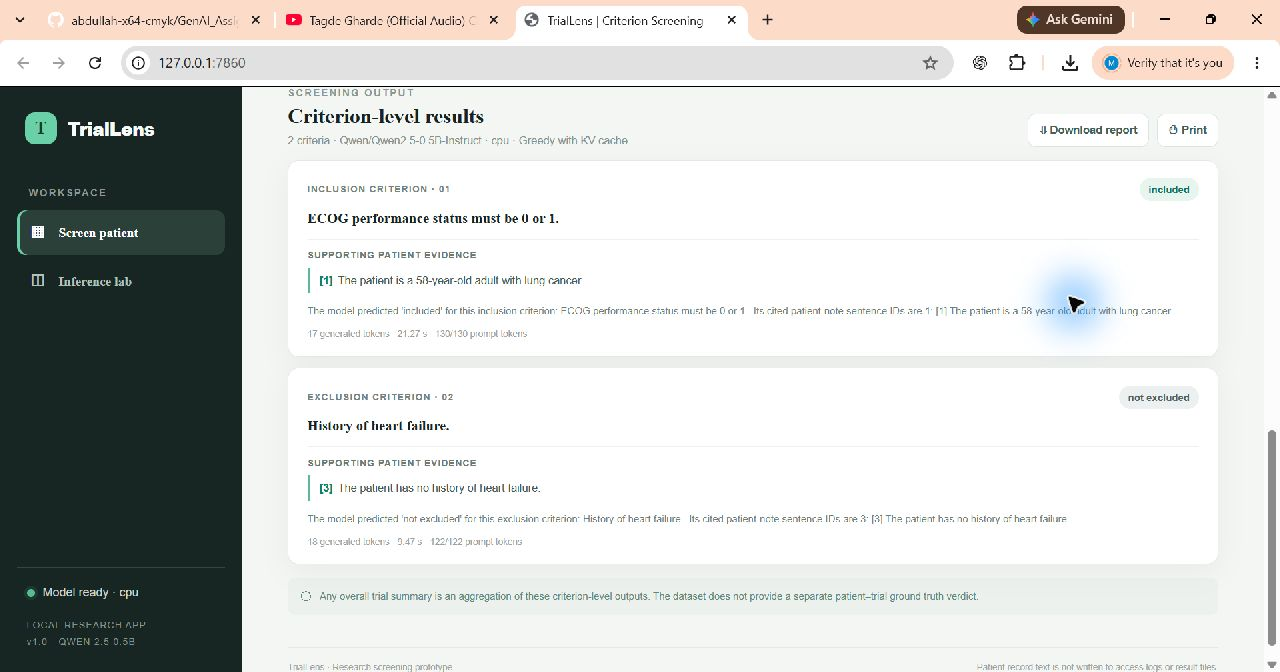
\includegraphics[width=.94\textwidth]{application_results.png}
\caption{Actual synthetic-patient screening output. ECOG is labeled included but cites the age/cancer sentence [1]; heart failure is labeled not excluded and correctly cites negative history [3]. This screenshot is a functional demonstration, not an additional accuracy experiment.}
\label{fig:app}\end{figure*}
}{}
\IfFileExists{figures/application_benchmarks.png}{
Figure~\ref{fig:appbench} shows how the evaluator can inspect saved inference measurements without executing notebook code.
\begin{figure*}[t]\centering
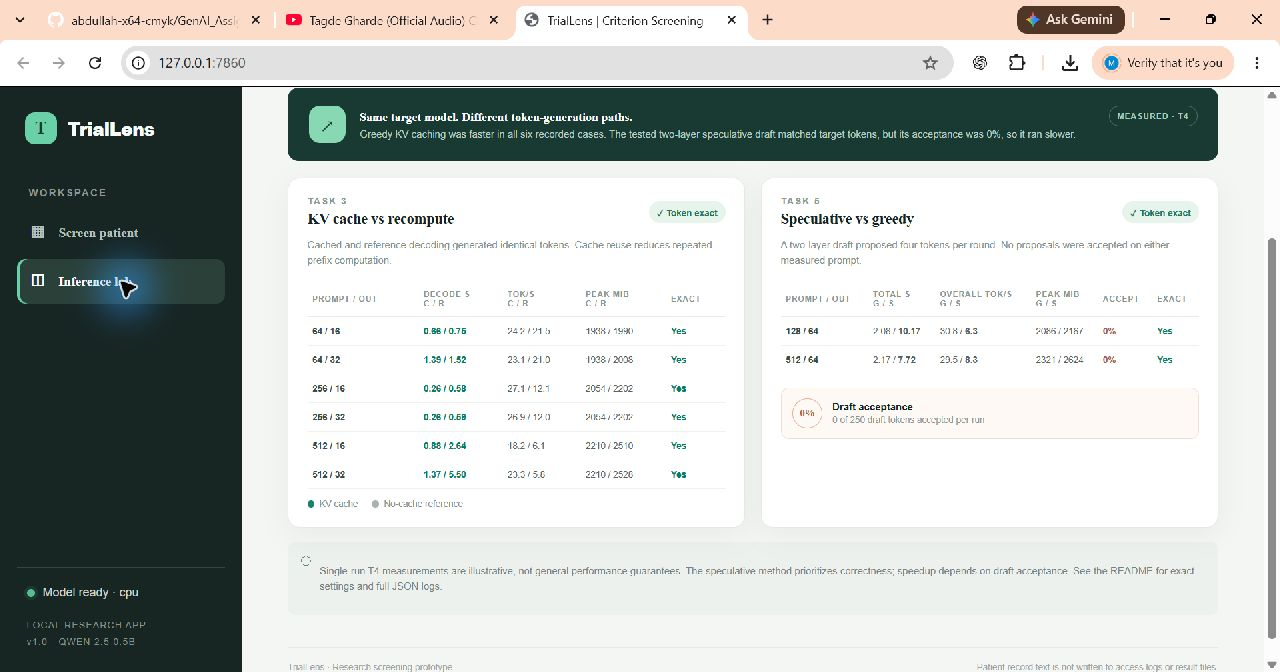
\includegraphics[width=.94\textwidth]{application_benchmarks.png}
\caption{Actual application inference-laboratory view, populated from archived T4 logs. The view exposes token equality, runtime, throughput, memory, and zero speculative acceptance.}
\label{fig:appbench}\end{figure*}
}{}
The readable HTML export was downloaded and inspected. The print control and live speculative path were not separately exercised in this browser demonstration; speculative correctness evidence comes from the dedicated benchmark. Text lookup verifies quotation origin, not semantic relevance.
\section{Limitations}

The benchmark is small and patient-grouped; performance estimates have substantial uncertainty. A generated rationale is not a verified clinical explanation; this task reports evidence IDs and should derive displayed evidence text from the source note. Small models may fail at negation, temporality, and implicit clinical reasoning. Although no truncation was observed in these runs, other longer notes may exceed the configured input budget. Base-model free-form outputs were not successfully normalized to the target schema, so the zero baseline scores should be interpreted with that limitation. The work is an educational screening prototype and must not determine clinical enrollment.

The eight test patients produce correlated criterion observations, and no repeated training seeds or patient-bootstrap confidence intervals were measured. Class imbalance and absence of excluded test cases restrict interpretation. The plain-prompt baseline is confounded by output-schema failure, and macro-F1 uses observed label unions that vary by group. Evidence IDs may be correct syntactically yet irrelevant, as the synthetic ECOG case shows; the audit explanation is not an independently verified rationale.

The microbenchmarks cover few validation-derived prompts on one T4. The successful cache rerun changes dtype and attention backend together, preventing attribution of preliminary mismatches to one cause. The draft is not separately trained and accepts no tokens in the measured workloads. Attention is an independent educational implementation rather than a fused kernel integrated into inference. Some final benchmark files retain summary equality assertions rather than full token traces. Training peak memory and an exact dependency lockfile were not archived. First-run downloads, CPU latency, long-note truncation, negation, and temporality remain practical limitations. No prospective clinical evaluation or clinician usability study was performed.
\section{Conclusion}

A compact open decoder adapted with LoRA improves criterion classification and evidence retrieval on the mandated patient-grouped benchmark, but macro-F1 of 0.398 and exclusion evidence recall of 0.125 expose substantial weaknesses. Explicit KV reuse matches the final reference greedy tokens and improves measured decoding efficiency. Tiled online softmax is numerically correct with a memory/runtime tradeoff; speculative decoding preserves the measured outputs but slows down with a weak draft. The browser application makes criterion decisions, exact citations, inference comparisons, and report export available without notebook execution. Future work should prioritize uncertainty preservation, evidence relevance, balanced patient-level evaluation, a trained draft, and repeated performance measurements. The prototype must not determine enrollment.
\section*{Source Project and Reproducibility}
Source code, the trained adapter archive, split manifest, experiment logs, application, and demonstration report are at \url{https://github.com/abdullah-x64-cmyk/GenAI_Assignment-2}. No paid GPU or proprietary inference API is compulsory. Figures and the per-class table regenerate from archived logs with \texttt{python report/generate\_figures.py}; no test inference is rerun. The Windows application launcher is \texttt{setup\_and\_run.bat}. The report source is \texttt{report/main.tex}.
\bibliographystyle{IEEEtran}
\bibliography{references}
\end{document}
